\documentclass{article}
\usepackage[margin=2.5cm, includefoot, footskip=30pt]{geometry}

\setlength{\parindent}{0em}
\setlength{\parskip}{1em}
\renewcommand{\baselinestretch}{1}

%%%%Packages%%%%
\usepackage{amsmath}
\usepackage{booktabs}
\usepackage{graphics}
\usepackage{multicol}
\usepackage{algorithm,algorithmic}
\usepackage{graphicx}
\usepackage{subcaption}
%%%%%%%%%%%%%%%%%

\setlength{\tabcolsep}{3pt}

\title{Applying modern data analysis techniques to tournament results of the
Iterated Prisoner's Dilemma.}
\date{}

\begin{document}

\maketitle

\section{Introduction}

According to Charles Darwin’s theory of evolution~\cite{oldroyd1986}, natural
selection is ruled by the survival of the fittest. However, in spite of all the
`selfish genes` it is observed that in interactions both social and biological
cooperation emerges. Individuals that cooperate more than other can even outperform
their population. Thus the following question arises: why cooperation emerges;
More over, how cooperative an individual must be to perform well in their respective
environment.

In the field of Game Theory the game of the Prisoner's Dilemma (PD) has been used
to explain the emerge of cooperative behaviour. The PD is a \(2\) player game
where both players have two strategies. They can either cooperate (C) or defect (D)
with one another. Their decisions are made simultaneously and independently.

The normal form representation of the game is given by matrix~\ref{matrix:pd}.

\begin{equation}\label{matrix:pd}
    \begin{bmatrix}
    (R,R) & (S,T)  \\
    (T,S) & (P,P)
    \end{bmatrix}
\end{equation}

where the payoffs \((R, P, S, T)\) are constrained by equations (\ref{eq:constrain_one})
and (\ref{eq:constrain_two}).

\begin{equation}\label{eq:constrain_one}
    T > R > P > S,
\end{equation}

\begin{equation}\label{eq:constrain_two}
    2R > T + S.
\end{equation}

Constraint~\ref{eq:constrain_one} ensures that D dominates the first action C
and constraint~\ref{eq:constrain_two} ensures that a social dilemma arises. That
is because the sum of the utilities to both players is best when they both cooperate.

Though not many insights can be gained from one shot game, complex behaviour that
allow further investigation arise in the repeated form; in the Iterated Prisoner's
Dilemma (IPD).

In the 1980’s, a political scientist called Robert Axelrod carried out a computer
tournament. Scholars from various disciplines were invited to submit strategies
in computer code and they would compete in a round robin tournament where the
strategy with the highest average score would be the winner. Axelrod’s tournament
has been used to explain how cooperation can be evolutionarily advantageous.

Strategies are a set of rules used to describe to a player how to play the IPD game.
The research of computer tournaments includes studying the interactions of such
strategies and the exploration of a strategy that dominates them all.


\section{Collecting data}

For performing a large number of computer tournaments the open source package
Axelrod Library~\cite{axelrodproject} is used. The package was introduced in 2015,
it is written in the programming language Python and it allow us to perform
a number of different tournaments with different strategies. The payoff values used in
Axelrod are \((3, 1, 0, 5)\) and the following type of tournaments have been performed.

There are several tournament types introduced in the literature that have not been
discussed.

\begin{enumerate}
    \item \textbf{Standard tournament}. A round robin tournament where
    the number of turns for each match can vary between 200 and 1. The tournament
    is repeated between 10 and 100 times.
    \item \textbf{Noisy tournament}. Similar to a standard tournament. A noisy
    tournament in a round robin tournament where noise is introduced. Noise is the
    probability that a players action is flipped. The probability of noise is
    ranging between 0 and 1.
    \item \textbf{Probabilistic ending tournament}. Similar to a standard tournament
    however in a probabilistic ending tournament the number of turns is not specified.
    There is a probability (ranges between 0 and 1) that the match will end in
    the next round. Probabilistic ending tournament will be referred to as
    probend hereupon.
    \item \textbf{Noisy and Probabilistic ending tournament}. A combination of
    noisy and probabilistic ending tournaments.
\end{enumerate}

The process for generating the data set is described by Algorithm~\ref{alg:tournaments}.
Every 20 iterations of a random seed a new sample is chosen. For each sample, for 20
repetitions random numbers of turns, repetitions of the tournament, the probability of
noise in the tournament and the probability of the game ending in after each interaction
are sampled.

For that set of parameters, four types of tournaments (as discussed above) are conducted.
A standard one, a noisy one, a probend one and lastly a probend with noise.

\begin{algorithm}
    \caption{Generating data}
    \label{alg:tournaments}
      \begin{algorithmic}[1]
        \FOR{seed \textbf{in} 10000}
            \IF{$seed \ mod \ 20 =0$}
                \STATE size $\gets$ random  size
                \STATE players $\gets$ random players
             \ELSE
                 \STATE turns $\gets$ random turns
                 \STATE repetitions  $\gets$  random  repetitions
                 \STATE noise  $\gets$ random  noise  probability
                 \STATE end  $\gets$  random end probability
                 \STATE standard results $\gets$ tournament(turns, players, repetitions) 
                 \STATE noise results $\gets$ tournament(turns, players, repetitions, noise)
                 \STATE probend results $\gets$ tournament(players, repetitions, end)
                 \STATE probend noise results $\gets$ tournament(players, repetitions, noise, end)
             \ENDIF
             \RETURN standard, noise, probend, probend noise results
        \ENDFOR
      \end{algorithmic}
\end{algorithm}

Once a tournaments is performed we export a summary of the performance
of each strategy in the tournament. In the following sections we discuss how we
manipulate the result set exported by Axelrod and hold a data analysis.

\section{Data preparation}

Each tournaments exports a summary of the results. These are separated by tournament
type. The structure of a single row of the results set is shown in
Table~\ref{table:result_set}. Name is the name of the strategy. Stochastic,
Memory depth and Use of arguments are characteristics of the given strategy.
The performance of the strategy is reflected by columns Rate, Median score, Rank and Wins.

The environment and the type of tournaments are captured by columns Noise, Probend,
Repetitions, Size and Turns. Note that when turns are non given the tournament is a
probabilistic ending one, and vise versa. Similarly, when Noise argument in non given
the tournament is known to be standard. Finally, when both Noise and Probend are
non zero then the tournament is an probabilistic and noisy tournament.

\begin{table}[htpb]
    \centering
    \resizebox{\columnwidth}{!}{%
    \begin{tabular}{ccccccccccccccccccccccccccccccccc}
    \toprule
    % columns
    Name & Stochastic & \multicolumn{1}{p{2cm}}{\centering Memory \\ depth} &
    \multicolumn{1}{p{2cm}}{\centering Use of \\ game} &
    \multicolumn{1}{p{2cm}}{\centering Use of \\ length} & CC rate &  CD rate &
    \multicolumn{1}{p{2cm}}{\centering Cooperation \\rating} & DC rate & DD rate &
    Median score &  Rank &  Wins &  Noise  &  Probend & Repetitions &  Seed & Size & Turns \\
    \midrule
    % first row
    Adaptive & False & inf & True & False & 0.195 &  0.214 & 0.409 & 0.279 & 0.310 &
    2.430 & 14 &  77.0 &  0.391 & NaN & 25.0 & 0.0 & 101.0 & 148.0 \\
    \bottomrule
    \end{tabular}}
    \caption{Result Set}
    \label{table:result_set}
\end{table}

Each types is explored separately. Figure~\ref{fig:cooperation_distributions} shows
the distributions of the cooperation rating for each type. As suggested probabilistic
ending tournaments are the most cooperative tournaments. Standard tournaments
appear to be most cooperative as well and any tournament which includes noise
the cooperation rating appears to follow a normalised distribution.

\begin{figure}
    \centering
    \begin{subfigure}{0.45\textwidth}
        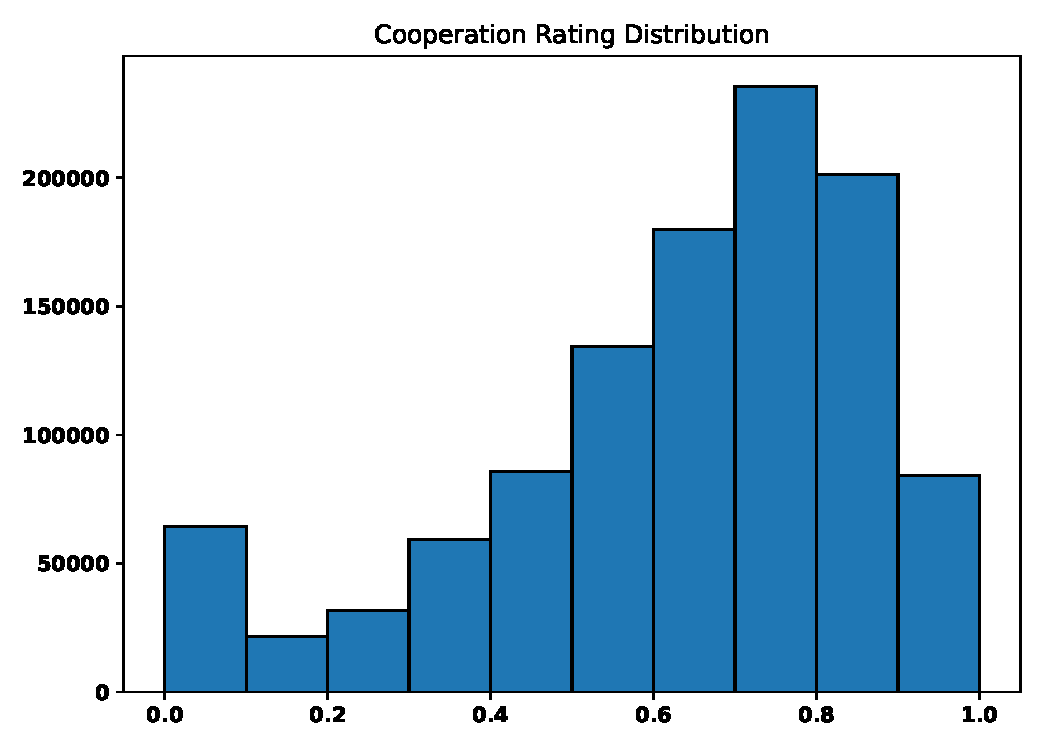
\includegraphics[width=\textwidth]{images/cooperation_distribution_std}
        \caption{Standard tournament type.}
    \end{subfigure}
    \begin{subfigure}{0.45\textwidth}
        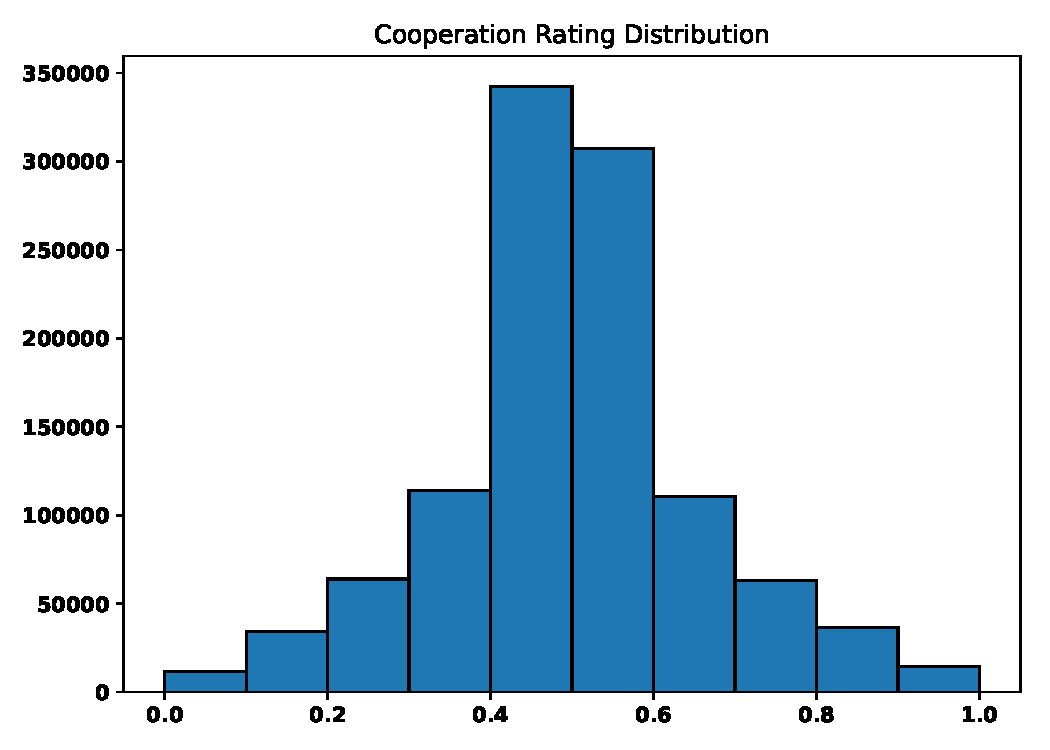
\includegraphics[width=\textwidth]{images/cooperation_distribution_noise}
        \caption{Noise tournament type.}
    \end{subfigure}
    \begin{subfigure}{0.45\textwidth}
        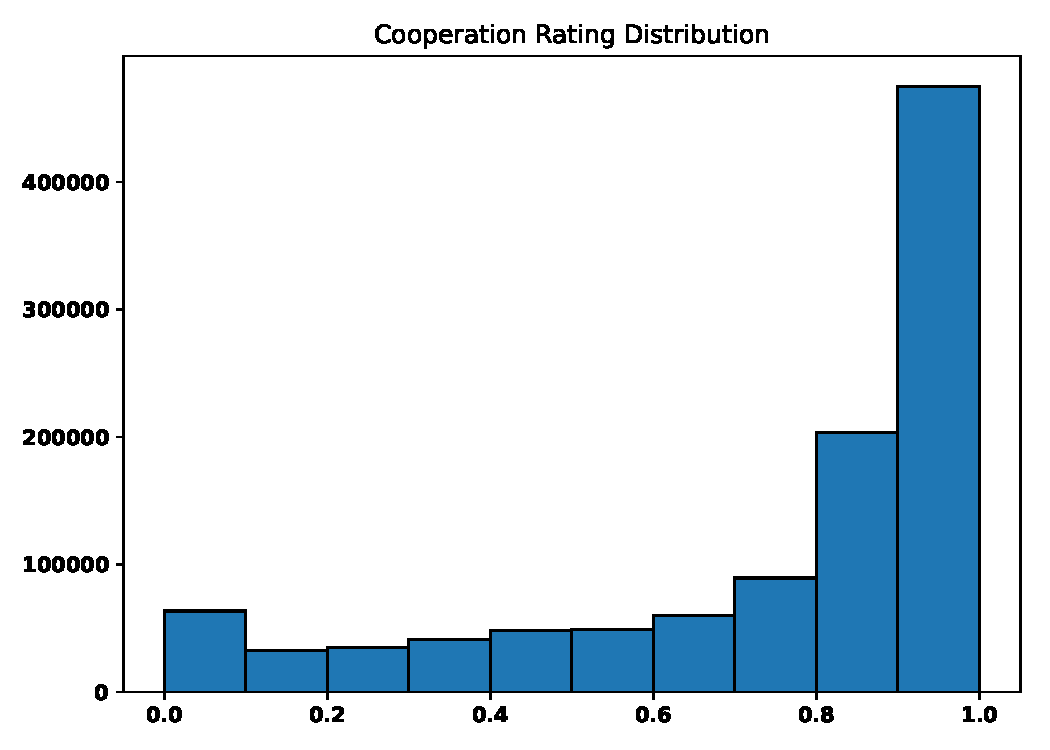
\includegraphics[width=\textwidth]{images/cooperation_distribution_probend}
        \caption{Probend tournament type.}
    \end{subfigure}
    \begin{subfigure}{0.45\textwidth}
        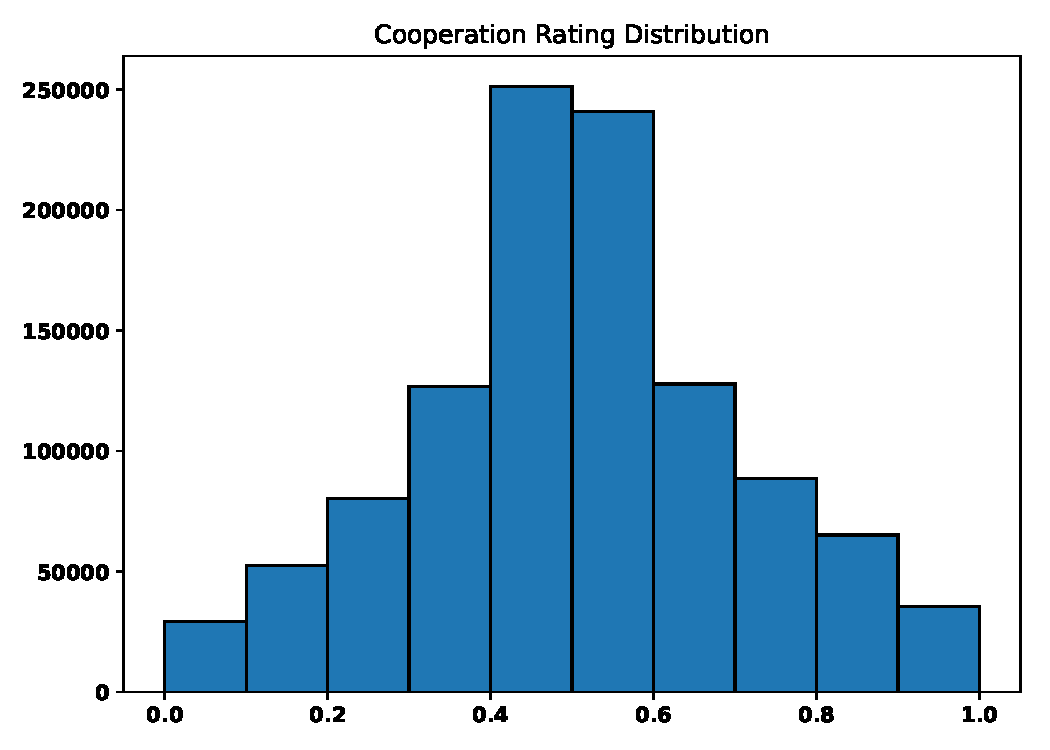
\includegraphics[width=\textwidth]{images/cooperation_distribution_noise_probend}
        \caption{Noise Probend tournament type.}
    \end{subfigure}
    \caption{Cooperation rating distribution.}\label{fig:cooperation_distributions}
\end{figure}

In this work each tournament type is studied individually. An individual data set
containing the following information is constructed for each type.

\begin{multicols}{2}
    \begin{itemize}
        \item tournament index \(i\)
        \item tournament size \(N_{i}\)
        \item maximum cooperation rating \(C^{*}_{r}\)
        \item minimum cooperation rating  \(\tilde{C_{r}}\)
        \item mean cooperation rating \(\bar{C_{r}}\)
        \item median cooperation rating \(\breve{C_{r}}\)
        \item standard deviation of the cooperating ratio \(\sigma\)
        \item \(C\) ratio of the winner \(C_{W}\)
        \item \(C\) ratio of the looser \(C_{L}\)
        \item \(C\) to \(CC\) rate of the winner
        \item \(C\) to \(CD\) rate of the winner
        \item \(C\) to \(DC\) rate of the winner
        \item \(C\) to \(DD\) rate of the winner
        \item normalised rank of maximum cooperator \(\bar{r_{C}}\)
        \item normalised rank of minimum cooperator \(\bar{r_{D}}\)
    \end{itemize}
    \end{multicols}

\section{Analysis}


\bibliographystyle{plain}
\bibliography{bibliography}
\end{document}